\documentclass[11pt]{article}
\usepackage{report}

\title{Monte Carlo Methods \\ lab 2}
\author{Jesper Vesterberg (jeve0010@student.umu.se)}

\date{\today}

\begin{document}
\begin{titlepage}
  \maketitle
  \thispagestyle{fancy}
  \lhead{
    Department\\
    Umeå Universitet
  }
  \rhead{\today}
  \begin{abstract}

  \end{abstract}
  \cfoot{
    Numerical Monte Carlo Methods\\
   	Supervisor: Peter Olsson 
  }
\end{titlepage}

\lhead{\theauthor}
\rhead{\thetitle\\\today}
\cfoot{\thepage}



\begin{thebibliography}{9}
\end{thebibliography}

\section{Universality}
In figure \ref{fig:mvsT} we can see how the magnetization is dependent on the temperature, using
the Wolff cluster method.
\begin{figure}[H]
	\centering
	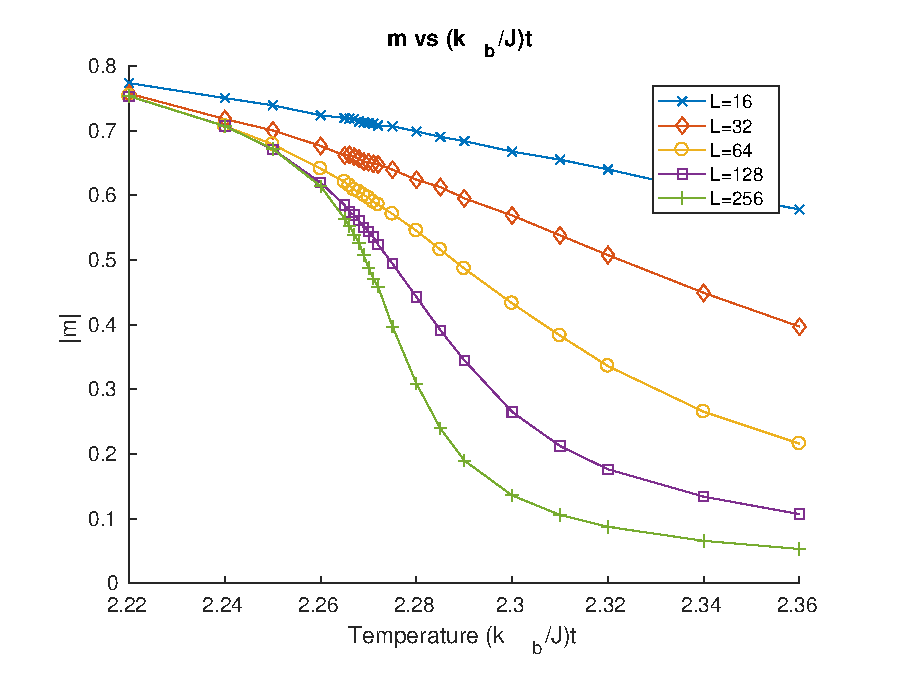
\includegraphics[width=0.9\textwidth]{mvsT}
	\caption{Looking at the magnetization at different temperatures using the Wolff cluster
method.}
	\label{fig:mvsT}
\end{figure}

\newpage
In figure \ref{fig:mlvsT} we can see how we are very close to the correct critical temperature in the
intersection, kind of like how we do with binder’s cumulant. Perhaps this is just an
coincident, perhaps not. It does in anyway clearly show, as in the previous picture, a
clearer drop around the critical temperature for larger systems.
\begin{figure}[H]
	\centering
	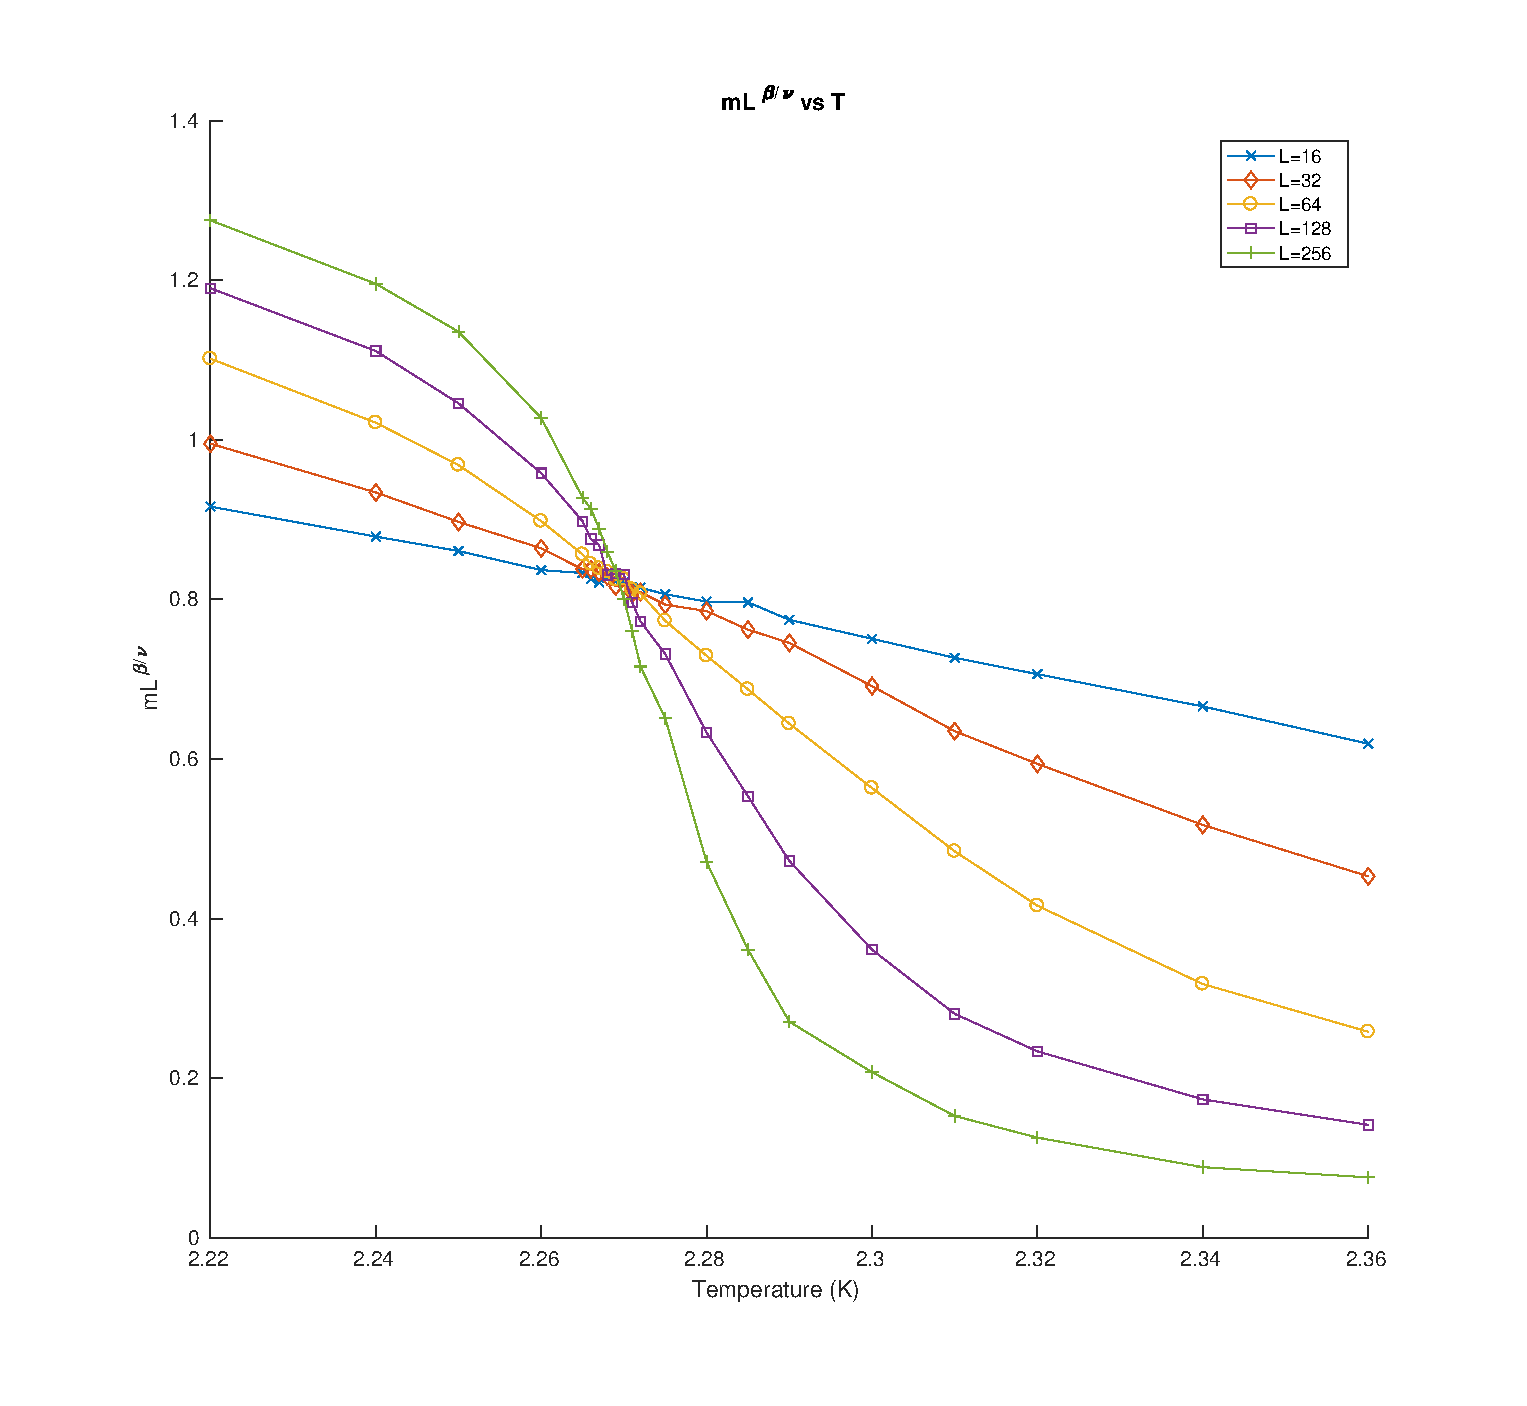
\includegraphics[width=0.9\textwidth]{mlvsT}
	\caption{The scaled magnetization plotted against the temperature}
	\label{fig:mlvsT}
\end{figure}

\newpage
In figure \ref{fig:mlvstl} we see how the scaling can be used to show you can find the behaviour at
an arbitrary size, when the system has only been simulated for one size.
\begin{figure}[H]
	\centering
	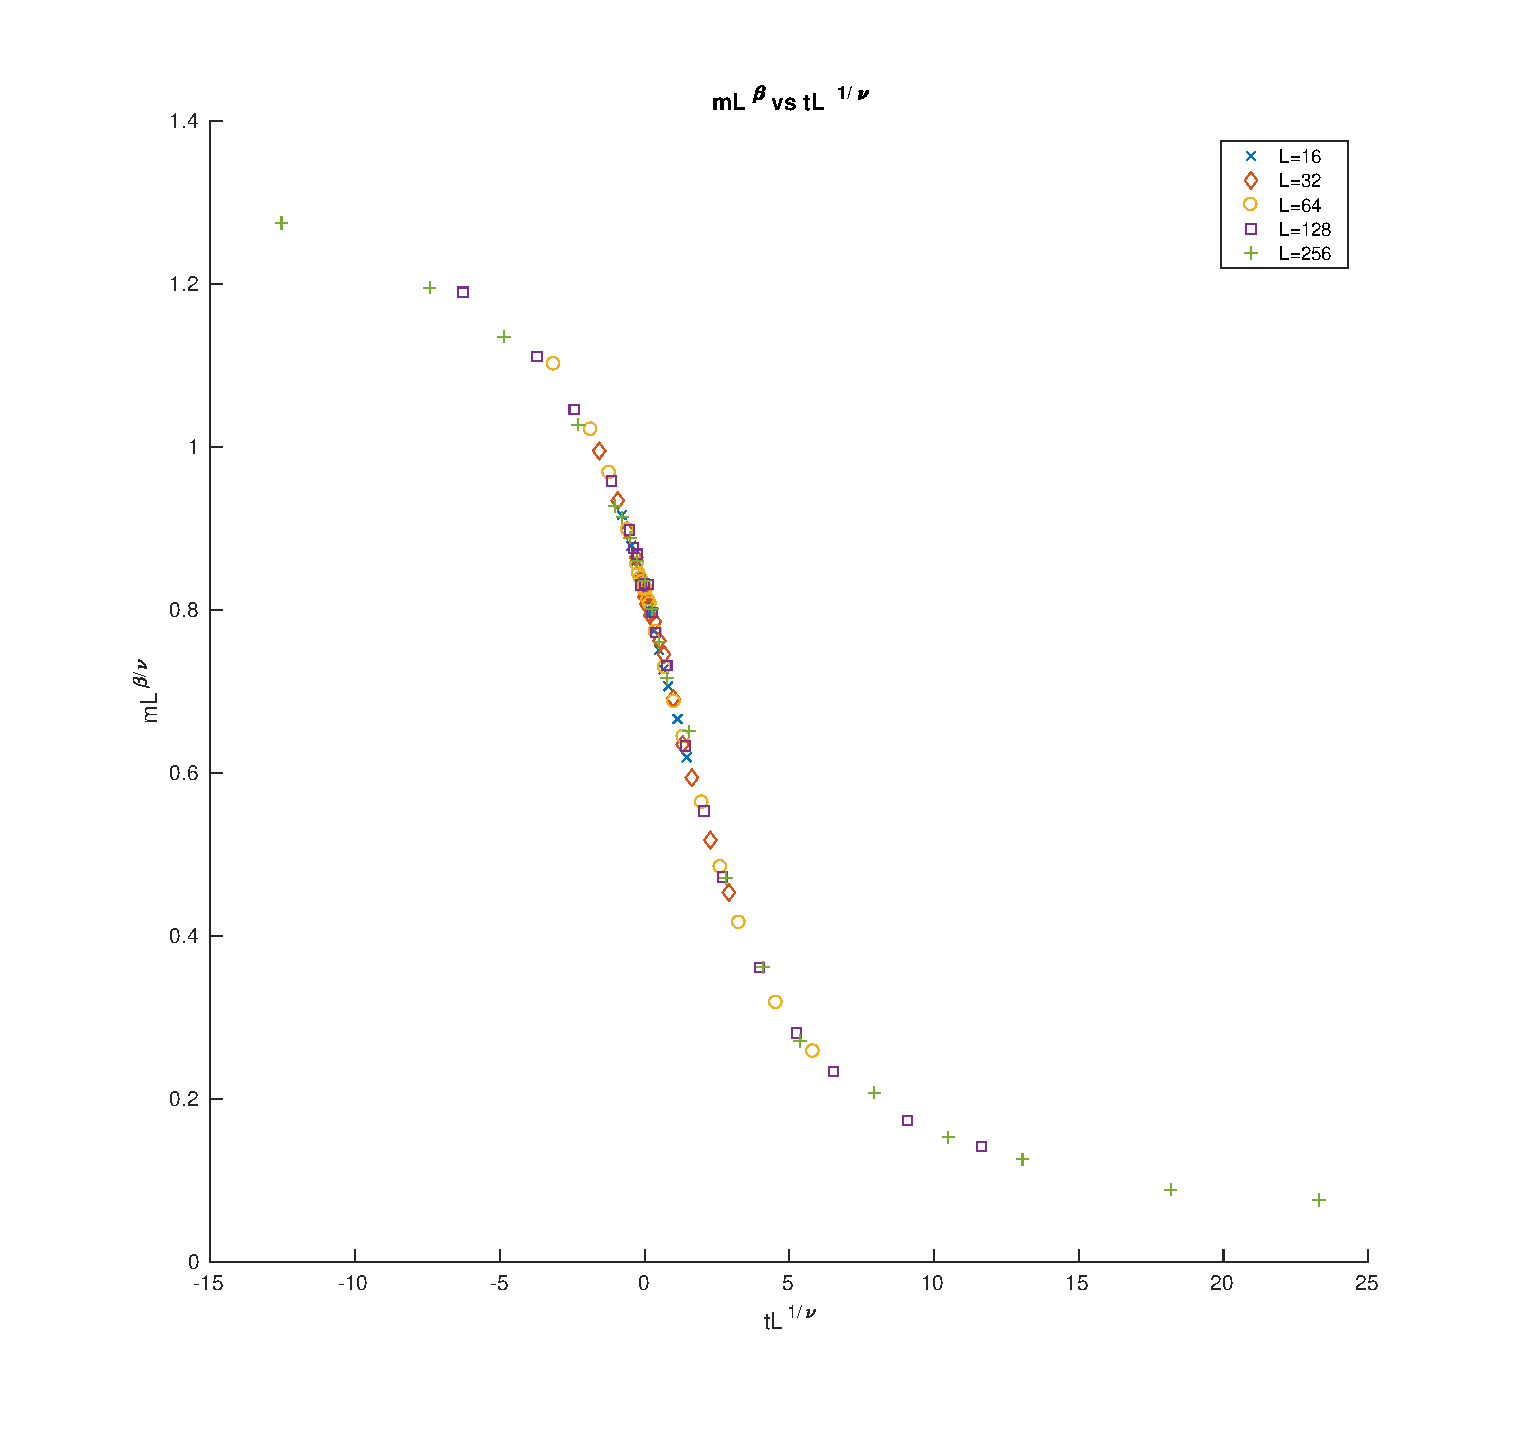
\includegraphics[width=0.9\textwidth]{mlvstl}
	\caption{Using the correct values for the universal constants $\upsilon$ and $\beta$ we get the
characteristic of the different system to collapse ontop of eachother.}
	\label{fig:mlvstl}
\end{figure}

\newpage
In figure \ref{fig:error} we can see how correct this assumption of the system behaving the same
for all system sizes with the correct scaling. We've zoomed in around the critical temperature and added the error bars in the plot.
\begin{figure}[H]
	\centering
	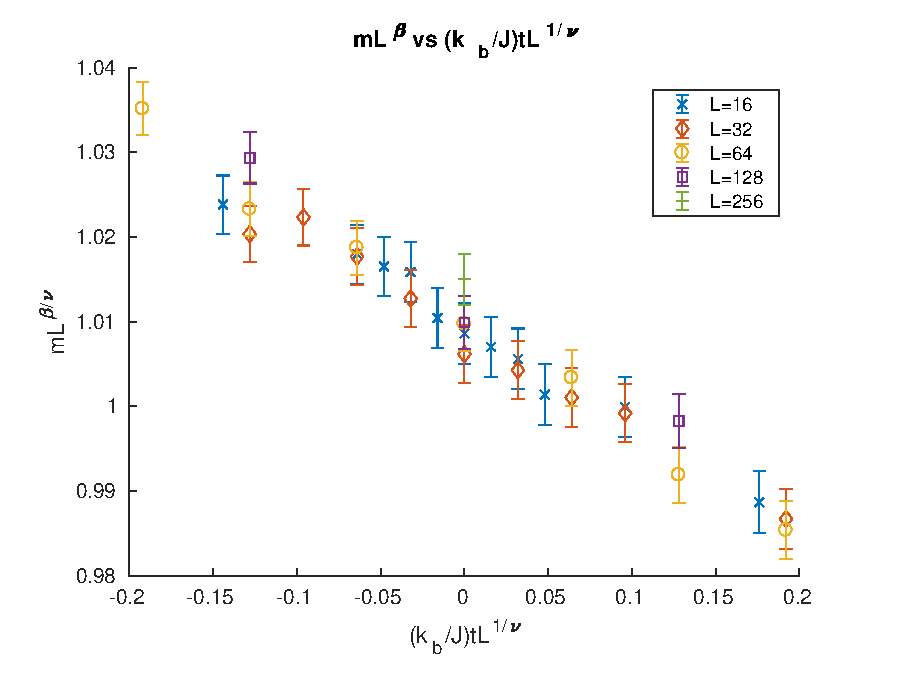
\includegraphics[width=0.9\textwidth]{error}
	\caption{Looking at the magnetization at different temperatures using the Wolff cluster
method.}
	\label{fig:error}
\end{figure}


\section{Binder's Cumulant}

In figure \ref{fig:cumulant} we can see how Binder's cumulant depends on temperature.
\begin{figure}[H]
	\centering
	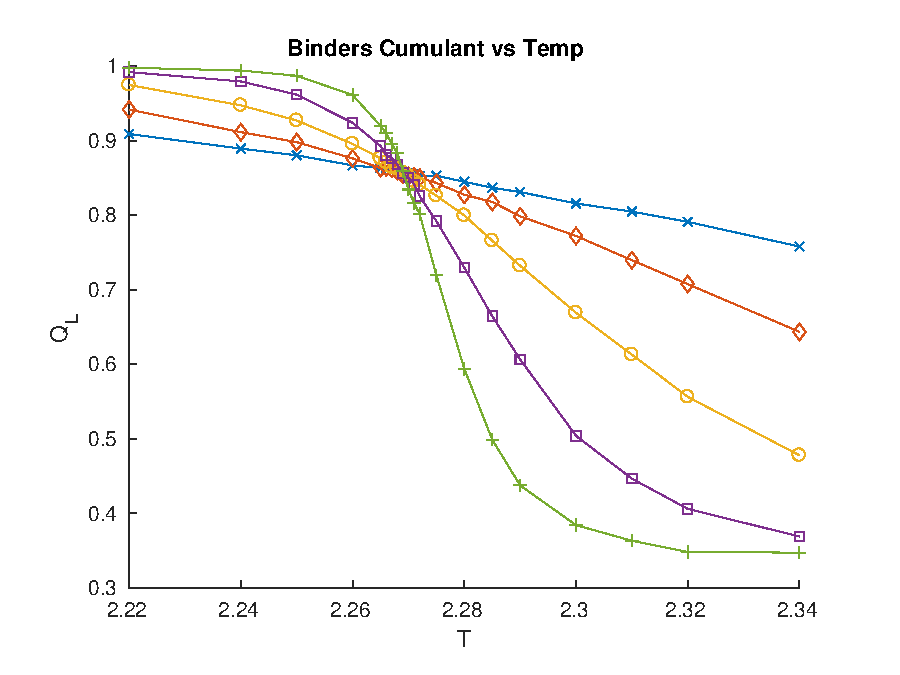
\includegraphics[width=0.9\textwidth]{cumulant}
	\caption{Looking at binder’s cumulant versus temperature to find the critical tempera-
ture.}
	\label{fig:cumulant}
\end{figure}

\newpage
Using the critical value we obtained in figure 5 we can collapse the cumulant function
by plotting in against $(T-T_c)L^{1 / \upsilon}$, as shown in figure \ref{fig:scaledtemp}.
\begin{figure}[H]
	\centering
	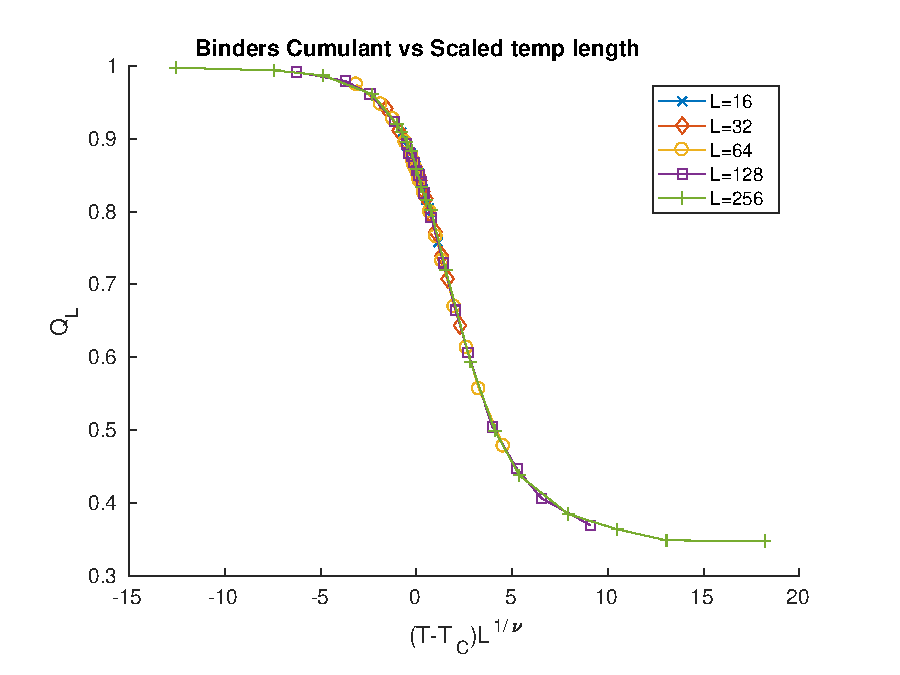
\includegraphics[width=0.9\textwidth]{scaledtemp}
	\caption{Binders cumulant as it depends on the scaled temperature}
	\label{fig:scaledtemp}
\end{figure}
\clearpage
\appendix
\section{Appendix}

\end{document}

